\documentclass[12pt,a4paper]{report}

\usepackage[utf8x]{inputenc}
\usepackage[left=2cm, right=2cm, top=5cm]{geometry}
\usepackage{enumitem}
\usepackage{fontspec}
\usepackage{pgf}
\usepackage{tikz}
\usepackage{amsmath}
\usepackage{algpseudocode}
\usetikzlibrary{arrows,automata}

\algblock[Name]{Start}{End}
\algblockdefx[NAME]{START}{END}
[2][Unknown]{Start #1(#2)}
{Ending}
\algblockdefx[NAME]{}{OTHEREND}
[1]{Until (#1)}

\usetikzlibrary{graphs, shapes, snakes, graphdrawing}
\usegdlibrary{layered, force}

\begin{document}

	\newcommand{\upon}[1]{\textbf{Upon} #1 \textbf{do}}

	\begin{titlepage}
		\centering
		{\scshape\LARGE Universidad Nacional Autónoma de México \par}
		\vspace{1cm}
		{\scshape\Large Computación Distribuida\par}
		\vspace{1.5cm}
		{\huge\bfseries Tarea 5\par}
		\vspace{.5cm}
		{\Large\itshape Edgar Quiroz Castañeda \par}
	    \vspace{.5cm}
		{\Large\itshape Jerónimo Almeida Rodríguez \par}
		\vfill
		 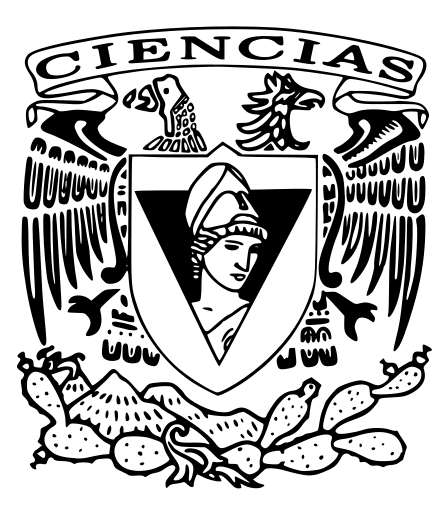
\includegraphics[width=0.5\textwidth]{escudo_f-ciencias.png}
		\vfill

		{\large Jueves 27 de septiembre del 2018 \par}
	\end{titlepage}

	\pagebreak
	\setlength{\voffset}{-0.75in}
	\setlength{\headsep}{5pt}

	\begin{enumerate}
		%Ejercicio 1
		\item {
			Considere la gráfica $G$. Propón retardos y ejecuta el algoritmo PIF con
			$p_1$ como raíz.\\

			La Figura 1 es la gráfica dada para el ejercicio.\\
			La Figura 2 es la misma gráfica con pesos asignados para simular retardos
			y con $p_1$ cómo raíz.\\
			De las Figuras 3-7 obtenemos la siguiente tabla:
			\begin{center}
				 \begin{tabular}{||c c c c||}
				 \hline
				 $r$ & \leftarrow & $p_1$ & $t_0$ \\
				 \hline
				 $p_1$ & \leftarrow & $p_6$ & $t_1$ \\
				 \hline
				 $p_1$ & \leftarrow & $p_2$ & $t_3$ \\
				 \hline
				 $p_6$ & \leftarrow & $p_5$ & $t_2$ \\
				 \hline
				 $p_2$ & \leftarrow & $p_2$ & $t_3$ \\
				 \hline
				 $p_6$ & \leftarrow & $p_4$ & $t_4$ \\ [1ex]
				 \hline
				\end{tabular}
			\end{center}
			De la cual podemos formar el árbol dirigido de la Figura 8, el cual nos
			muestra el árbol óptimo de propagación de PIF.\\
			De esto, sumando el peso de las aristas de cada rama del árbol, tenemos que
			la propagación tarda 4 unidades de tiempo y todo el algoritmo $PIF$, ahora con
			retroalimentación tarda 8 unidades de tiempo.
			\newpage
			\begin{figure}[h!]
				\begin{center}
					\begin{tikzpicture}[-,>=stealth',shorten >=1pt,auto,node distance=2.8cm,
		                    semithick]
					\tikzstyle{every state}=[fill=none,draw=black,text=black]

					\node[state] (A)                    {$p_1$};
					\node[state] (B) [above right of=A] {$p_2$};
					\node[state] (C) [right of=B] 		{$p_3$};
					\node[state] (D) [below right of=C] {$p_4$};
					\node[state] (E) [below right of=A] {$p_6$};
					\node[state] (F) [above right of=E] {$p_5$};

					\path 	(A) edge              node {} (B)
					        	edge              node {} (F)
								edge 			  node {} (E)
					    	(B) edge 			  node {} (C)
					        	edge              node {} (D)
					    	(C) edge              node {} (D)
					    	(E) edge 			  node {} (D)
								edge 			  node {} (F)
							(F) edge 			  node {} (D);
					\end{tikzpicture}
					\caption{Grafica Inicial.}
				\end{center}
			\end{figure}

			\begin{figure}[h!]
				\begin{center}
					\begin{tikzpicture}[-,>=stealth',shorten >=1pt,auto,node distance=2.8cm,
		                    semithick]
					\tikzstyle{every state}=[fill=none,draw=black,text=black]

					\node[state] (A)                    {$p_1$};
					\node[state] (B) [above right of=A] {$p_2$};
					\node[state] (C) [right of=B] 		{$p_3$};
					\node[state] (D) [below right of=C] {$p_4$};
					\node[state] (E) [below right of=A] {$p_6$};
					\node[state] (F) [above right of=E] {$p_5$};

					\path 	(A) edge              node {2} (B)
					        	edge              node {3} (F)
								edge			  node {1} (E)
					    	(B) edge 			  node {1} (C)
					        	edge              node {3} (D)
					    	(C) edge              node {2} (D)
					    	(E) edge 			  node {3} (D)
								edge 			  node {1} (F)
							(F) edge 			  node {2} (D);
					\end{tikzpicture}
					\caption{Grafica Inicial con Pesos Elegidos Aleatoriamente para Simular
							 Retardos. Con $p_1$ inicializado cómo raíz en $t_0=0$}
				\end{center}
			\end{figure}

			\begin{figure}[h!]
				\begin{center}
					\begin{tikzpicture}[-,>=stealth',shorten >=1pt,auto,node distance=2.8cm,
		                    semithick]
					\tikzstyle{every state}=[fill=none,draw=black,text=black]

					\node[state] (A)                    {$p_1$};
					\node[state] (B) [above right of=A] {$p_2$};
					\node[state] (C) [right of=B] 		{$p_3$};
					\node[state] (D) [below right of=C] {$p_4$};
					\node[state] (E) [below right of=A] {$p_6$};
					\node[state] (F) [above right of=E] {$p_5$};

					\path 	(A) edge              node {2} (B)
					        	edge              node {3} (F)
								edge[blue]		  node {1} (E)
					    	(B) edge 			  node {1} (C)
					        	edge              node {3} (D)
					    	(C) edge              node {2} (D)
					    	(E) edge 			  node {3} (D)
								edge 			  node {1} (F)
							(F) edge 			  node {2} (D);
					\end{tikzpicture}
					\caption{Primer paso de la ejecución en $t_1=1$.}
				\end{center}
			\end{figure}

			\begin{figure}[h!]
				\begin{center}
					\begin{tikzpicture}[-,>=stealth',shorten >=1pt,auto,node distance=2.8cm,
		                    semithick]
					\tikzstyle{every state}=[fill=none,draw=black,text=black]

					\node[state] (A)                    {$p_1$};
					\node[state] (B) [above right of=A] {$p_2$};
					\node[state] (C) [right of=B] 		{$p_3$};
					\node[state] (D) [below right of=C] {$p_4$};
					\node[state] (E) [below right of=A] {$p_6$};
					\node[state] (F) [above right of=E] {$p_5$};

					\path 	(A) edge[green]              node {2} (B)
					        	edge              node {3} (F)
								edge[blue]			  node {1} (E)
					    	(B) edge 			  node {1} (C)
					        	edge              node {3} (D)
					    	(C) edge              node {2} (D)
					    	(E) edge		      node {3} (D)
								edge[green] 	  node {1} (F)
							(F) edge 			  node {2} (D);
					\end{tikzpicture}
					\caption{Segundo paso de la ejecución en $t_2=2$.}
				\end{center}
			\end{figure}

			\begin{figure}[h!]
				\begin{center}
					\begin{tikzpicture}[-,>=stealth',shorten >=1pt,auto,node distance=2.8cm,
		                    semithick]
					\tikzstyle{every state}=[fill=none,draw=black,text=black]

					\node[state] (A)                    {$p_1$};
					\node[state] (B) [above right of=A] {$p_2$};
					\node[state] (C) [right of=B] 		{$p_3$};
					\node[state] (D) [below right of=C] {$p_4$};
					\node[state] (E) [below right of=A] {$p_6$};
					\node[state] (F) [above right of=E] {$p_5$};

					\path 	(A) edge[green]       node {2} (B)
					        	edge[red]         node {3} (F)
								edge[blue]		  node {1} (E)
					    	(B) edge[red]		  node {1} (C)
					        	edge              node {3} (D)
					    	(C) edge              node {2} (D)
					    	(E) edge 			  node {3} (D)
								edge[green] 	  node {1} (F)
							(F) edge 			  node {2} (D);
					\end{tikzpicture}
					\caption{Tercer paso de la ejecución en $t_3=3$.}
				\end{center}
			\end{figure}

			\begin{figure}[h!]
				\begin{center}
					\begin{tikzpicture}[-,>=stealth',shorten >=1pt,auto,node distance=2.8cm,
		                    semithick]
					\tikzstyle{every state}=[fill=none,draw=black,text=black]

					\node[state] (A)                    {$p_1$};
					\node[state] (B) [above right of=A] {$p_2$};
					\node[state] (C) [right of=B] 		{$p_3$};
					\node[state] (D) [below right of=C] {$p_4$};
					\node[state] (E) [below right of=A] {$p_6$};
					\node[state] (F) [above right of=E] {$p_5$};

					\path 	(A) edge[green]       node {2} (B)
					        	edge[red]         node {3} (F)
								edge[blue]		  node {1} (E)
					    	(B) edge[red]		  node {1} (C)
					        	edge              node {3} (D)
					    	(C) edge              node {2} (D)
					    	(E) edge[violet]	  node {3} (D)
								edge[green] 	  node {1} (F)
							(F) edge        	  node {2} (D);
					\end{tikzpicture}
					\caption{Cuarto paso de la ejecución en $t_4=4$.}
				\end{center}
			\end{figure}

			\begin{figure}[h!]
				\begin{center}
					\begin{tikzpicture}[-,>=stealth',shorten >=1pt,auto,node distance=2.8cm,
		                    semithick]
					\tikzstyle{every state}=[fill=none,draw=black,text=black]

					\node[state] (A)                    {$p_1$};
					\node[state] (B) [above right of=A] {$p_2$};
					\node[state] (C) [right of=B] 		{$p_3$};
					\node[state] (D) [below right of=C] {$p_4$};
					\node[state] (E) [below right of=A] {$p_6$};
					\node[state] (F) [above right of=E] {$p_5$};

					\path 	(A) edge[green]       node {2} (B)
					        	edge[red]         node {3} (F)
								edge[blue]		  node {1} (E)
					    	(B) edge[red]		  node {1} (C)
					        	edge[orange]      node {3} (D)
					    	(C) edge[orange]   	  node {2} (D)
					    	(E) edge[violet]	  node {3} (D)
								edge[green] 	  node {1} (F)
							(F) edge[orange]	  node {2} (D);
					\end{tikzpicture}
					\caption{Quinto paso de la ejecución en $t_5=5$.}
				\end{center}
			\end{figure}
			\begin{figure}[h!]
				\begin{center}
					\begin{tikzpicture}[-,>=stealth',shorten >=1pt,auto,node distance=2.8cm,
		                    semithick]
					\tikzstyle{every state}=[fill=none,draw=black,text=black]

					\node[state] (A)                    {$p_1$};
					\node[state] (B) [above right of=A] {$p_2$};
					\node[state] (C) [right of=B] 		{$p_3$};
					\node[state] (D) [below right of=C] {$p_4$};
					\node[state] (E) [below right of=A] {$p_6$};
					\node[state] (F) [above right of=E] {$p_5$};

					\path 	(A) edge		      node {2} (B)
					        	edge	          node {1} (E)
					    	(B) edge			  node {1} (C)
					    	(E) edge			  node {3} (D)
								edge		 	  node {1} (F);
					\end{tikzpicture}
					\caption{Quinto paso de la ejecución en $t_5=5$.}
				\end{center}
			\end{figure}
			\newpage
		}

		%Ejercicio 2
		\item {
			En la Ciudad de México varios puntos de control (nodos) fueron agregados.\\
			Cada uno de estos puntos tiene información de cuantas personas viven
			dentro de cierto diámetro. \\
			Un punto (raíz) de la delegacion Benito Juárez quiere recolectar la
			información de todos los puntos de control. \\
			Escribe un algoritmo para que cada nodo recolecte la información de sus
			hijos para enviarsela al padre sin repetirla.\\

			\begin{algorithmic}[1]
				\Function{collectInformation}{population}
					\State $children \ \leftarrow \emptyset$
					\State $nonChildren \ \leftarrow \emptyset$
					\State $totalPopulation \ \leftarrow population$
					\If{$p_{id}\ =\ root$}
						\State $parent\ \leftarrow\ root$
						\State $send$ $M$ to all neighbors
					\Else
						\State $parent\ \leftarrow\ \bot$
					\EndIf
					\State \upon{receiving $M$ from $p$}
					\Start
						\If{$parent\ =\ \bot$}
							\State $parent\ \leftarrow\ p$
							\State $send$ $M$ to all neighbors except $p$
						\Else
							\State $send$ $nack$ to $p$
						\EndIf
					\End
					\State \upon{receiving $nack$ from $p$}
					\Start
						\State $nonChildren\ \leftarrow\ nonChildren\ \cup\ {p}$
					\End\\
					\textbf{When} $children\ \cup\ nonChildren\ =\ allMyNeighbours
							\	\textbf{do}$
					\Start
						\If{$p_{id}\ =\ root$}
							\State $return$ $totalPopulation$
						\Else
							\State $send\ (ack, totalPopulation)\ to\ parent$
						\EndIf\\
					\textbf{End}\\
					\upon{receiving $(ack, pPopulation)$ from $k$}
					\Start
						\State $add\ k\ to\ children$
						\State $totalPopulation = totalPopulation + pPopulation$
					\End
					\End
				\EndFunction
			\end{algorithmic}
			El algoritmo es básicamente $PIF$, que ya se sabe que es correcto. \\
			El propósito de $PIF$ es primero enviar
			un mensaje a todos los nodos. Cada nodo lleva la cuenta de quien es su
			padre y quienes son sus hijos. El padre es el nodo del que reciben el mensaje
			por primera vez, por lo que sólo tiene uno.\\
			Cuando recibe confirmación de todos sus hijos, lo que se cumple por
			vacuidad cuando los nodos son hojas, entonces envía un mensaje de
			confirmación a su padre.\\
			En esta modificación del algoritmo, cada nodo representa un punto de control.\\
			Cada nodo recibe como parámetro la población que vive en su radio.\\
			Los mensajes de confirmación se cambian por parejas, donde el primer elemento
			es el mensaje de confirmación y el segundo es la población acumulada de
			ese nodo y todos los hijos de ese nodo.\\
			Cada vez que se recibe ese mensaje de alguno de los hijos, la
			población acumulada del hijo su suma a la población acumulada del padre.
			Entonces, lo que se envía a su padre es la población inicial del nodo más
			la población acumulada de cada uno de sus hijos.\\
			Como sólo se envía una vez la población acumulada al padre, entonces se
			garantiza que nunca se cuenta dos veces a la misma población.\\
			Al terminar la raíz, el valor que devuelve es la suma de la población
			acumulada de todos sus hijos más su población, que es la población total.\\
			}


		%Ejercio 3
		\item{
			Demuestre por inducción que en el algoritmo PI, cada nodo $v$ recibe el
			mensaje $M$ por primera vez en a lo más $d(root, v)$.\\

			\textbf{Caso Base: }\\
			Supongamos que $v$ es el primer nodo en recibir el me nwsaje en tiempo $t$
			Supongamos que $d(r,v)\neq t$ entonces, $d(r,v) < t$ ya que no hay pesos
			negativos en las aristas, entonces, existe $T=(r=v_0,v_1,...,v_k=v)$ tal que
			\[t'= \sum_{i=0}^{k-1} w(v_i,v_{i+1})\  <t,\ v_i\neq v_k\]
			Suponemos que no hay aristas de peso cero.\\
			$d(v_0,v_1)<t$, lo que implica que $v$ recibe $M$ antes.\\
			\textbf{Hipótesis de Inducción:}\\
			Supongamos que para los primeros $k$ vértices en llegarles el mensaje
			se cumple que $d(r,v)=t(v)$\\
			\textbf{Paso Inductivo: }\\
			P.D. Si $v'$ es el $k-1$ en recibir el mensaje, entonces $d(r,v') = t(v')$
			Sea $T=(r=v_0,v_1,...,v_n=v'$ de longitud mínima, Entonces
			\[\sum_{i=0}^{n-1}w(v_i,v_{i+1})\ =\ d(r,v'),\ T'= (r=v_0,v_1,...,v_{n-1})\]
			es de longitud mínima.
			$v_{n-1}$ recibió $M$ antes $t(v_{n-1})=d(r,v_{n-1})$ por \textbf{H.I.}.
			Entonces,
			\[t(v_n) \leq t(v_{n-1})+w(v_{n-1},v_n)=w(T')+w(v_{n-1},v_n)=w(T)=d(r,v')
				\geq t(v')\]
			Por lo tanto, $t(v')=d(r,v')$\\
			Afirmamos entonces que $d(r,v')\geq t(v')$.\\
			Supongamos que $d(r,v')<t(v')$, entonces existe $T=(r=v_0,...,v_s=v')$
			tal que $w(T)<t(v')$. Entonces, $r$ podría mandar a $M$ a través de $T$
			en un tiempo menor. Esto contradice lo que habíamos supuesto y por lo tanto
			la propiedad se cumple.
		}
		%Ejercio 4
		\item{
			Se dice que una digráfica $G = (V, E)$ tiene raiz $r \in V$ y cada
			vértice $v \in V$ es alcanzable desde $r$, es decir, existe un camino
			dirigido alcanzable desde $r$ (un camino dirigido que empieza en $r$ y
			termina en $v$).\\
			Una digráfica $G$ es un  ́arbol dirigido si tiene raíz y la versión no dirigida
			de $G$ es un árbol. Demuestra el siguiente teorema:\\

			\textbf{Teorema 1}\\
			Sea G una digráfica. Las siguientes condiciones son equivalentes
			\begin{enumerate} [label = \alph*)]
				\item {
					$G$ es un árbol dirigido.\\
				}
				\item {
					$G$ tiene una raíz desde la cual hay un único camino dirigido a
					vértice.\\
				}

				\item{
					$G$ tiene una raíz $r$ para la cual $\delta(r)_{in} = 0$, y para cualquier
					otro vértice $v$, $\delta_{in}(v) = 1$.\\
				}

				\item{
					$G$ tiene una raíz $r$ y el quitar cualquier arista interumpe la
					condición.\\
				}
				\item{
					La versión no dirigida de $G$ es conexa y $G$ tiene un vértice $r$ para
					el cual $\delta_{in}(r) = 0$ mientras que para cualquier otro vértice
					$v$ $\delta(v)_{in} = 1$.\\
				}
			\end{enumerate}

			\begin{itemize}
				\item[$a \implies b$]{

					Sea $G$ un árbol dirigido. Por definición, significa que tiene una raíz,
					esto es un vértice desde el cuál hay un camino a cualquier otro vértice de
					$G$.\\
					Sólo falta ver que ese camino es único.\\

					Primero, notemos que esos camino son trayectorias, pues si uno de estos
					caminos, dígamos $c = (r = v_1, ..., v_n)$ tuviera un vértice repetido,
					digamos $v_i = v_j, i < j$, entonces $c' = (r = v_1, ..., v_i = v_j, ... v_n)$
					sería un cliclo en la versión no dirigida de $G$, por lo que la versión
					no dirigida de $G$ no sería un árbol.\\

					Luego, tomemos dos de estas trayectorias $c_1 = (r = v_1, ..., v_n = u)$ y
					$c_2 = (r = w_1, ..., w_m = u)$ y supongamos que son diferentes.\\
					Sea $v_i = w_j \in V$ el primer vértice no raíz que hay en común entre
					$c_1$ y $c_2$, cuya existencia se puede garantizar porque en el caso
					extremo este vértice es $u$.\\
					Entonces, en la versión no dirigida de $G$, consideremos el camino
					$c_3 = (r = v_1, v_2, ..., v_i = w_j, w_{j-1}, ..., w_2, w_1 = r)$.\\
					Cómo los $v_k$ provienen de una trayectoria, entonces no se repiten entre
					sí, al igual que los $w_l$.\\
					Además, como $v_i = w_j$ es el primer vértice en común entre las
					trayectorias originales, entonces los $v_k$ y  los $w_l$ no tienen ningún
					otro vértice en común.
					Entonces $c_3$ es una trayectoria, y comienza  y termina en el mismo
					vertice, por lo que es un ciclo.\\
					Entonces, la versión no dirigida de $G$ no es un árbol, lo cuál no es
					posible. Esta contradicción surge de suponer que $c_1$ y $c_2$ eran
					diferentes. Entonces, cualesquiera dos caminos entre la raiz y un mismo
					vértice son en realidad el mismo.\\
					Entoces el camino dirigido entre la raíz y cualquier vértice es único.\\
				}

				\item[$b \implies c$]{
					Sea $G$ una digráfica dirigida con una raíz $r$ y cuyos caminos entre la raíz y
					cualquier otro vértice son únicos.\\
					Veamos que $\delta(r)_{in} = 0$. Por contradicción, supongamos que
					$\delta(r)_{in} < 0$. Entonces sea $v \in N^+(r)$. Como $r$ es raíz,
					entonces existe un camino, $c = (r = v_1, ..., v)$. \\
					Entonces, $c' = (r = v_1, ..., v, r)$ contiene un ciclo en la versión no
					dirigida de $G$, pero esta debe de er un árbol.\\
					Entonces $\delta(r)_{in} = 0$.\\
					Luego, veamos cuál es el grado interior de los demás vértices.
					Sea $w \in V$. Como hay un camino $c_1 = (r = w_1, ..., w_n = w)$,
					entonces al menos un vértice $w_{n-1}$ incide en $w$, por lo que
					$\delta(w)_{in} \geq 1$.\\
					Luego, supongamos que $\delta(w)_{in} > 1$. Entonces sean
					 $u_1, u_2 \in N^+(w), u_1 \neq u_2$.\\
					Como $r$ es raíz, entonces existen caminos únicos $s_1 = (r = x_1, ..., x_n = u_1)$
					y $s_2 = (r = y_1, ..., y_n = u_2)$.\\
					Tanto $s_1$ como  $s_2$ inciden es $w$, entonces
					$s_1 = (r = x_1, ..., x_n = u_1, w)$ $s_2 = (r = y_1, ..., y_n = u_2, w)$
					son dos caminos de la raiz a $w$ diferentes, pues al menos $x_n = u_1 \neq y_n = u_2$.
					Pero los caminos desde la raíz son únicos. Esta contradicción surge de
					asumir que $\delta(w)_{in} > 1$.\\
					Por lo tanto, $\delta(w)_{in} = 1$.\\
				}


				\item[$c \implies d$]{
					Sea $G$ una digráfica que tiene una raíz $r$ para la cual $\delta(r)_{in} = 0$,
					y para cualquier otro vértice  $v \in V$, $\delta_{in}(v) = 1$.\\
					Cómo $G$ tiene raíz, sólo falta demostrar que $G-\{e\}, e \in E$ no tiene
					raíz.\\
					Sea $e = (v, w) \in E$. Si $v = r$, entonces $(v, w)$ era el camino único
					entre $v$ y $w$. Entonces ya no hay un camino entre $v$ y $w$. Entonces
					$r$ ya no es raíz.\\
					Si $r \neq w$, $\delta_{in}(w) = 1$, esto es que sólo un vértice
					incide en $w$, y cómo $v$ incide en $w$, por lo que $v$ es el único vértice
					que incide en $w$.\\
					Por esto en $G-\{e\}$, ningún vértice incide en $w$. Por lo tanto
					no hay ningún camino que llega a $w$.
					Por lo tanto, $G-\{e\}$ no puede tener raíz.\\
				}

				\item[$d \implies e$]{
					Sea $G$ una digráfica que tiene un raíz $r$ y cualquier arista que quites
					hace que $G$ ya no tenga raíz.\\
					Consideremos la versión no dirigida de $G$, digamos $G'$. Entonces, se
					mantiene que existen caminos $c_u = (u_0 = r, ..., u_n = u)$
					entre $r$ y cualquier otro vértice $u$ de $G'$.\\
					Entonces, entre cualquier $v, w \in V(G')$ se tiene que
					$c = (v = v_n, v_{n-1}, ..., v_1=r=w_1, w_2, ..., w_m)$ es un camino entre
					$v$ y $w$ en $G'$, pues no es dirigida.\\
					Por lo tanto, la verisón no dirigida $G'$ de $G$ es conexa.\\
					Luego, veamos que $\delta_{in}(r) = 0$.
					Supongamos que no, entonces $\delta_{in}(r) \geq 0$. Entonces sea
					$v \in N^+(r)$, por lo que $(v, r)\in E$.\\
					Consideremos a $G - {(v, r)}$, que no debe de tener raíz, por lo que debe
					de existir algún vértice $w$ para el que todo camino en $G$ contenía a $(v, r)$.
					Sea $c = (r = u_1, u_2, ..., u_k = v, u_{k+1} = r, ..., u_n = w)$ uno de
					esos caminos, y que sea de longitud mínima.\\
					Entonces, $c' = (u_{k+1} = r, u_{k+1} = r, ..., u_n = w)$ es un camino entre
					$r$ y $w$ de longitud menos a $c$. Esta contradicción surge de asumir que
					todos los caminos entre $r$ y $v$ pasaban por $(r, v)$. Entonces debe existir
					algún camino que no pasaba por $(r, v)$ en $G$. Entonces, en $G - {(v, r)}$
					sí hay un camino entre $r$ y $w$. Entonces $r$ sigue siendo raíz, pero esto
					no es posible. Esto surge de suponer que $\delta_{in}(r) \geq 0$.
					Entonces $\delta_{in}(r) = 0$.\\
					Ahora veamos que $v$ $\delta(v)_{in} = 1$ para cualquier vértice diferente
					de $r$.\\
					Supongamos que no, entonces sea $(w, v), (u, v) \in E, w \neq u$.\\
					Como $r$ es raíz, entonces existen $c_1 = (r = u_1, ..., u_n = u, v)$ y
					$c_2 = (r = w_1, ..., w_n=w, v)$, digamos de longitud mínima. Notemos que
					son trayectorias, pues de repetir alguna vértice $a$ se podría
					crear otro camino que no incluya a todos los vértices en la sucesión entre
					la primera y la segunda aparición de $a$ que tendría longitus menor.\\
					Consideremos $G - {(w, v)}$, que no debe de tener raíz. Entonces debe de
					existir algún vértice $x$ tal que todos sus caminos en $G$ pasan por
					$(w, v)$. Sea $c_3 = (r = x_1, ..., x_j = w, v = x_{j+1}, ..., x_n = x)$
					unos de esos caminos, y de longitud mínima.\\
					Pero tenemos que $c_4 = (r = u_1, ..., u_n = u, v = x_{j+1}, x_{j+2}, ..., x_n = x)$
					es un camino entre $r$ y $x$, y como ambos son trayectorias y ambos contienen
					a $v$ y en esa aparición de $v$ no está $w$ pegado a $v$, entonces no
					contiene a $(w, v)$, lo cual no es posible. Esta contradicción surge de
					suponer que todos los caminos pasan por $(w, v)$. Entonces hay un camino
					entre $r$ y $x$ en  $G - {(w, v)}$, por lo que $r$ sigue siendo raíz en
					$G - {(w, v)}$, lo cuál no es posible.\\
					Esto surge de suponer que $v$ $\delta(v)_{in} > 1$.\\
					Por lo tanto, $v$ $\delta(v)_{in} = 1$ para cualquier $v$ diferente de la
					raíz.\\
				}

				\item[$e \implies a$]{
					Sea $G$ digráfica tal que la versión no dirigida de $G$ es conexa y $G$
					tiene un vértice $r$ para el cual $\delta_{in}(r) = 0$ mientras que para
					cualquier otro vértice $v$ $\delta(v)_{in} = 1$.\\
					Primero, veamos que $r$ es raíz.\\
					Como la versión no dirigida de $G$ es conexa, entones ahí existe un camino
					entre $r$ y cualquier otro vértice $v$, digamos $c = (r = v_1, ..., v_n = v)$.
					Veamos que este también es un camino entre $r$ y $v$ en $G$.\\
					Como $\delta_{in}(r) = 0$, entonces $r$ no puede tener vértices que le incidan,
					por lo tanto $(r, v_2) \in V(G)$. Y como $\delta(v)_{in} = 1$, y $v_2$ ya
					tiene una arista que le incide, debe de pasa que $(v_2, v_3) \in V(G)$.\\
					Y así sucesivamente. Entonces $(v_j, v_{j+1}) \in V(G), 0 \leq j < n$.\\
					Entonces, efectivamente $c$ es un camino entre $r$ y $v$ en $G$.\\
					Por lo tanto, existe un camino entre $r$ y cualquier vértice $v$.\\
					Entonces $r$ es raíz.\\
					Luego, veamos que la versión no dirigida de $G$ es un árbol.\\
					Como la versión no dirigida de $G$, $G'$ es conexa, sólo falta mostrar que
					$G'$ no tiene ciclos.\\
					Supongamos que tiene algún ciclo $c = (v_1, ..., v_n, v_1)$ en $G'$.\\
					Entonces, es $G$ este ciclo puede ser de varias formas. Digamos $c$ también
					es un ciclo válido en $G$, es decir que $(v_j, v_{j+1}) \in E(G)$.\\
					No puede incluir a $r$, pues de ser así un vértice incidiría en $r$, lo
					cual no es posible. Entonces, para tener un camino entre $r$ y alguno de
					los vértices de $c$, alguno de los vértices del camino debe de tener una
					adyacencia con un vértice que no sea del ciclo, además del vértice al que
					es adyacente dentro del ciclo. Entonces tendría al menos dos vértices que
					le son adyacentes, lo cual no es posible. Entonces el $c$ no puede estar
					en $G'$.\\
					Entonces, si los no se cumple que $(v_j, v_{j+1}) \in E(G), 0 \leq j < n$,
					entonces existe algún $v_j \in V(G)$ que no cumples que
					$(v_j, v_{j+1})\in E(G)$. Y como $v_j$ y $v_{j+1}$ son adyacente en $G'$,
					tiene que pasar que $(v_{j+1}, v_j)\in E(G)$.
					Pero además $(v_{j-1}, v_j)\in E(G)$, por lo que $\delta(v)_{in} \geq 2$.
					Lo cuál no es posible, por lo que $c$ no puede existir en $G'$.
					Entonces, $G´$ es acíclica, por lo que es un árbol.
					Entonces, $G$ tiene raíz y su versión acíclica es un árbol, por lo que es
					$G$ es un árbol dirigido.
				}
			\end{itemize}

		}
	\end{enumerate}
\end{document}
